\subsection{棱锥、圆锥的体积}\label{subsec:2-9}
\begin{enhancedline}

前一节,我们用\hyperref[zgyl]{祖暅原理}求出了柱体(棱柱、圆柱)的体积。
为了求出锥体的体积公式,我们首先研究等底面积等高的任意两个锥体体积之间的关系。

取任意两个锥体,设它们的底面积都是 $S$,高都是 $h$(图 \ref{fig:ltjh-2-63})。

\begin{figure}[htbp]
    \centering
    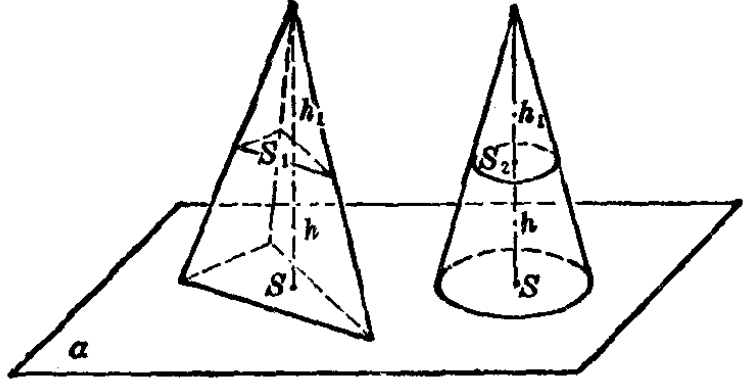
\includegraphics[width=10cm]{../pic/ltjh-ch2-63.png}
    \caption{}\label{fig:ltjh-2-63}
\end{figure}

把这两个锥体放在同一平面 $\alpha$ 上,这时它们的顶点都在和平面 $\alpha$ 平行的同一个平面内。
用平行于平面 $\alpha$ 的任意平面去截它们,截面分别与底面相似。 设截面和顶点的距离是 $h_1$,
截面面积分别是 $S_1$、$S_2$,那么

$\because$ \quad $\dfrac{S_1}{S} = \dfrac{h_1^2}{h^2}$, \quad $\dfrac{S_2}{S} = \dfrac{h_1^2}{h^2}$,

$\therefore$ \quad $\dfrac{S_1}{S} = \dfrac{S_2}{S}$, \quad  $S_1 = S_2$。

根据\hyperref[zgyl]{祖暅原理},这两个锥体的体积相等。由此我们得到下面的定理:

\begin{dingli}[定理][dl:zhuiti-tjxd]
    等底面积等高的两个锥体的体积相等。
\end{dingli}

现在,我们来证明三棱锥的体积公式。

\begin{dingli}[定理][dl:slzhui-tj]
    如果三棱锥的底面积是 $\bm{S}$,高是 $\bm{h}$,那么它的体积是
    \begin{center}
        \framebox[10em]{$\bm{V_\text{三棱锥} = \exdfrac{1}{3} Sh}$。}
     \end{center}
\end{dingli}

已知:三棱锥 1($A'{-}ABC$)的底面积是 $S$,高是 $h$。

求证: $V_\text{三棱锥} = \exdfrac{1}{3} Sh$。

\zhengming 把三棱锥 1 以 $\triangle ABC$ 为底面、$AA'$ 为侧棱补成一个三棱柱,
然后再把这个三棱柱分割成三个三棱锥,就是三棱锥 1 和另两个三棱锥 2、3(图 \ref{fig:ltjh-2-64})。

\begin{figure}[htbp]
    \centering
    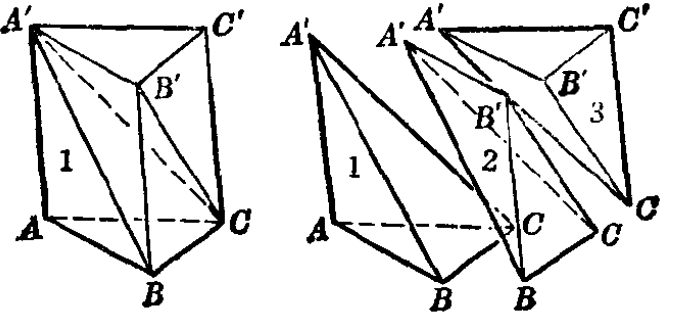
\includegraphics[width=10cm]{../pic/ltjh-ch2-64.png}
    \caption{}\label{fig:ltjh-2-64}
\end{figure}

三棱锥 1、2 的底 $\triangle ABA'$、$\triangle B'A'B$ 的面积相等,高也相等(顶点都是 $C$);
三棱锥 2、3 的底 $\triangle BCB'$、$\triangle C'B'C$ 的面积相等,高也相等(顶点都是 $A'$),

$\therefore$ \quad $V_1 = V_2 = V_3 = \exdfrac{1}{3} V_\text{三棱柱}$。

$\because$ \quad $V_\text{三棱柱} = Sh$,

$\therefore$ \quad $V_\text{三棱锥} = \exdfrac{1}{3} Sh$。

最后,因为和一个三棱锥等底面积等高的任何锥体都和这个三棱锥的体积相等,所以我们得到下面的定理:

\begin{dingli}[定理][dl:zhuiti-tj]
    如果一个锥体(棱锥、圆锥)的底面积是 $\bm{S}$,高是 $\bm{h}$,那么它的体积是
    \begin{center}
        \framebox[10em]{$\bm{V_\text{锥体} = \exdfrac{1}{3} Sh}$。}
    \end{center}
\end{dingli}


\begin{tuilun}[推论][tl:yuanzhui-tj]
    如果圆锥的底面半径是 $\bm{r}$,高是 $\bm{h}$,那么它的体积是
    $$ \bm{V_\text{圆锥} = \exdfrac{1}{3} \pi r^2 h} \juhao $$
\end{tuilun}


\liti 如图 \ref{fig:ltjh-2-65},已知:三棱锥 $A{-}BCD$ 的侧棱 $AD$ 垂直于底面 $BCD$,侧面 $ABC$ 与底面所成的角为 $\theta$。

求证: $V_\text{三棱锥} = \exdfrac{1}{3} S_{\triangle ABC} \cdot AD \cos\theta$。

\begin{wrapfigure}[4]{r}{5.5cm}
    \centering
    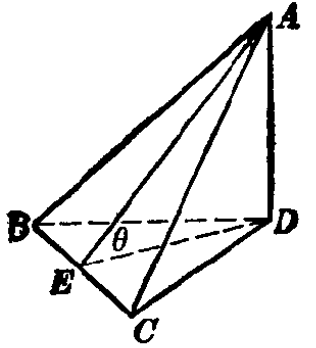
\includegraphics[width=4.5cm]{../pic/ltjh-ch2-65.png}
    \caption{}\label{fig:ltjh-2-65}
\end{wrapfigure}

\zhengming 在平面 $BCD$ 内,作 $DE \perp BC$,垂足为 $E$,连结 $AE$,
$DE$ 就是 $AE$ 在平面 $BCD$ 上的射影。根据\hyperref[dl:scx]{三垂线定理},$AE \perp BC$。

$\therefore$ \quad $\angle AED = \theta$。

$\begin{aligned}
    V_\text{三棱锥} &= \exdfrac{1}{3} S_{\triangle BCD} \cdot AD \\
        &= \exdfrac{1}{3} \times \exdfrac{1}{2} BC \cdot ED \cdot AD \\
        &= \exdfrac{1}{3} \times \exdfrac{1}{2} BC \cdot AE \cos\theta \cdot AD \\
        &= \exdfrac{1}{3} S_{\triangle ABC} \cdot AD \cos\theta \juhao
\end{aligned}$


\liti 一块正方形薄铁板的边长是 22 cm,以它的一个顶点为圆心,边长为半径画弧,沿弧剪下一个扇形,
用这块扇形铁板围成一个圆锥筒,求它的容积(保留两位有效数字)。

\jie 如图 \ref{fig:ltjh-2-66},扇形弧长是 $\exdfrac{1}{4} \cdot 44\pi = 11\pi$。
因此,所作的圆锥筒底的周长 $2 \pi r = 11\pi$。\\
解得 \quad $r = 5.5$。

因为母线长是 22 cm,所以圆锥的高

$h = \sqrt{22^2 - 5.5^2} \approx 21.3$。

$V_\text{圆锥} = \exdfrac{1}{3} \pi \times 5.5^2 \times 21.3 \approx 6.7 \times 10^2 \; (\lflm)$。

答:所求圆锥筒的容积约为 $670\;\lflm$。

\begin{figure}[htbp]
    \centering
    \begin{minipage}[b]{9cm}
        \centering
        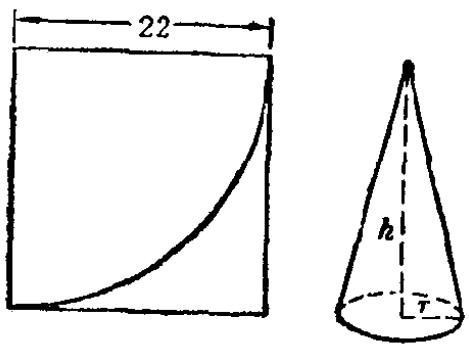
\includegraphics[width=9cm]{../pic/ltjh-ch2-66.png}
        \caption{}\label{fig:ltjh-2-66}
    \end{minipage}
    \qquad \qquad
    \begin{minipage}[b]{5cm}
        \centering
        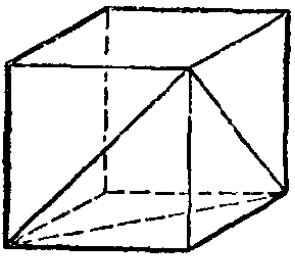
\includegraphics[width=5cm]{../pic/ltjh-ch2-subsec9-lx-01.png}
        \caption*{(第 1 题)}
    \end{minipage}
\end{figure}


\begin{lianxi}

\xiaoti{如图,将长方体沿相邻三个面的对角线截去一个三棱锥。这个三棱锥的体积是长方体体积的几分之几?}

\xiaoti{已知:圆锥的底面周长是 $c$,高是 $h$。 求证:这个圆锥的体积 $V$ 可以近似地表示为
    $V \approx \left(\exdfrac{c}{6}\right)^2 h$。
}

\end{lianxi}

\end{enhancedline}

